\documentclass[12pt, oneside]{article}
\usepackage[letterpaper, margin=1in]{geometry}
\usepackage[english]{babel}
\usepackage[utf8]{inputenc}
\usepackage{amsmath}
\usepackage{amsfonts}
\usepackage{amssymb}
\usepackage{tikz}
\usepackage{tkz-fct}

\usepackage{fancyhdr}
\pagestyle{fancy}
\fancyhf{}
\rhead{\thepage \\Name: \hspace{1.5in}.\\}
\lhead{BECA / Dr. Huson / 11.2 Algebra 2 \\* 23 May 2018 \\* \textbf{Pretest: Regents practice problems}}

\vspace{1cm}

\renewcommand{\headrulewidth}{0pt}

\title{Problem set template}
\author{Chris Huson}
\date{May 2018}

\begin{document}
%\maketitle

\subsubsection*{\\* \textnormal{Graph carefully using pencil}}

\begin{enumerate}

\item Given the periodic function $f(x)=\sin x$. 
\begin{enumerate}
    \item Using the calculator table function, complete the $y$ values.
    \begin{tabular}{r|r}
    x & $y=\sin(x)$\\ 
    \hline 
    $-1$ & \\[5pt]
    $0$ & \\[5pt]
    $1$ & \\[5pt]
    $1.5$ & \\[5pt]
    $2$ & \\[5pt]
    $3$ & \\[5pt]
    $4$ & \\[5pt]
    $4.5$ & \\[5pt]
    $5$ & \\[5pt]
    $6$ & \\[5pt]
    $7$ & \\ 
    \end{tabular}
    \item Graph the function on the grid below.
\end{enumerate}
\begin{center}
    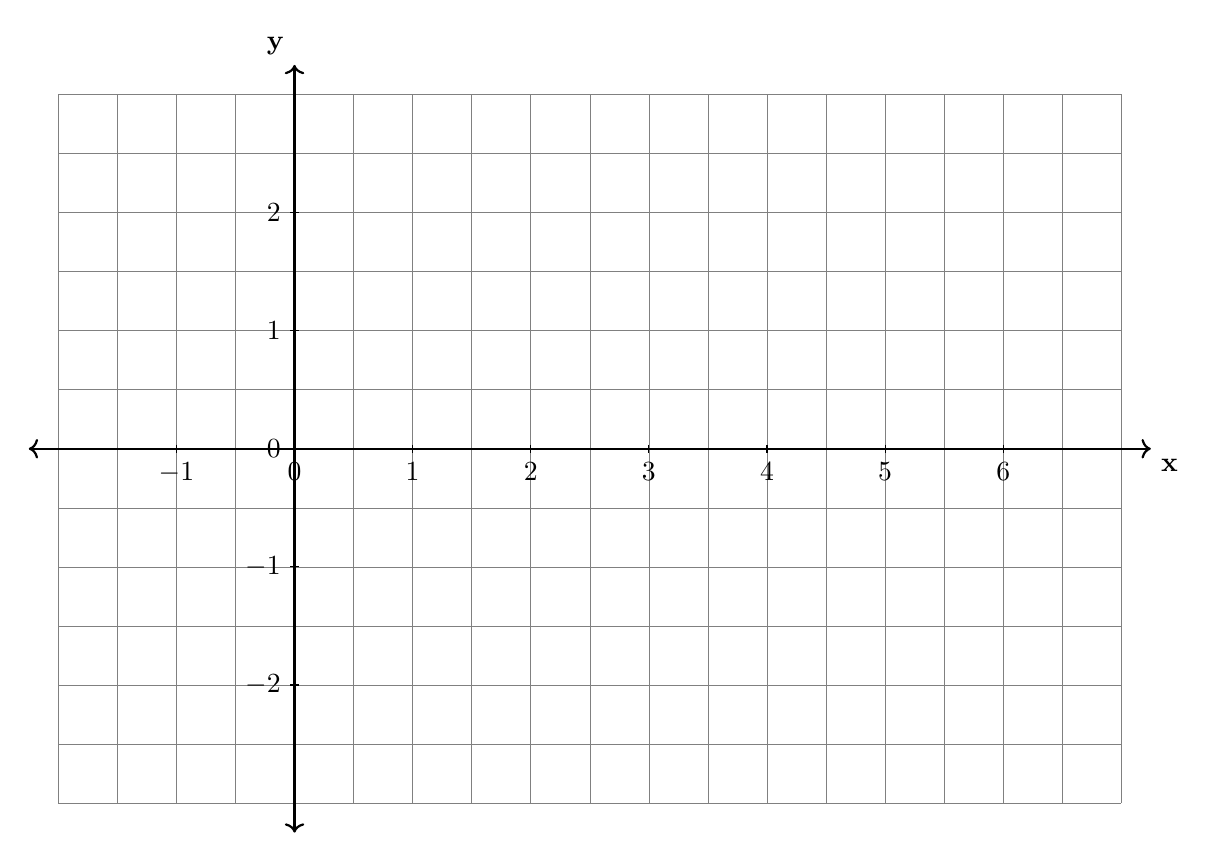
\begin{tikzpicture}[scale=6/4]
    \draw[step=0.5cm,gray,very thin] (-2,-3) grid (7,3);
    \draw[thick,<->] (-2.25,0) -- (7.25,0) node[anchor=north west] {\textbf{x}};
    \draw[thick,<->] (0,-3.25) -- (0,3.25) node[anchor=south east] {\textbf{y}};
    \foreach \x in {-1, 0, 1, 2, 3, 4, 5, 6} \draw (\x cm,1pt) -- (\x cm,-1pt) node[anchor=north] {$\x$};
    \foreach \y in {-2, -1, 0, 1, 2} \draw (1pt,\y cm) -- (-1pt,\y cm) node[anchor=east] {$\y$};
    %\foreach \y in {-5} \draw (1pt,\y cm) -- (-1pt,\y cm) node[anchor=east] {-50};    \tkzInit[xmin=-5,xmax=5,ymin=-7,ymax=7,ystep=1]   
%    \tkzFct[color=black,thick,<->,domain = -3.4:7] {0.1*(x*x-4)*(x-5)};
    \end{tikzpicture}
\end{center}

\newpage

\item Simplify the expression $(1 - 2i)^2$, where $i$ is the imaginary unit. \\*[1.25in]

\item Given $i$ is the imaginary unit, $(2-yi)^2$ in simplest form is what?  \\*[1.25in]%Alg2 Regents Jun2016


\item Write $\sqrt{x^3} \bullet \sqrt{x}$ as a single term with a rational exponent.\\*[1in]

\item When $b>0$ and $d$ is a positive integer, the expression $\displaystyle \left(3b \right)^\frac{2}{d}$ is equivalent to what expressed as a radical? \\*[1in]%Alg2 Regents Jun2016 multiple choice

\item What does $\displaystyle \left( \frac{8x^3}{y^6} \right)^\frac{2}{3}$ equal?

\newpage
\item The zeros of a cubic polynomial function $f$ are  $-2, 4, \text{ and } 6$. The polynomial has a negative leading coefficient, $a<0$. Sketch a graph of $y = f(x)$ on the grid below.\\*
\begin{center}
    
\begin{tikzpicture}
    \draw[step=0.25in,gray,very thin] (0,0) grid (12.7,12.7);
    \end{tikzpicture}
\end{center}
Write an equation for $f(x)$ in factored form, assuming the leading coefficient is negative one.\\*[30pt]


\newpage
\item Given: $f(x)=3x^2+ x - 2$ and $g(x)=2x-1$\\*[5pt]
Express $f(x) \bullet g(x) + 2x$ as a polynomial in standard form. \\*[3in]


\item Algebraically determine the values of $h$ and $k$ to correctly complete the identity stated below.
\[2x^3-5x^2+12x-5=(2x-1)(x^2-hx+k)\] %\\*[3in]


\newpage
\item What are the zeros for $f(x)=x^4-4x^3-9x^2+36x$? \\*[1in]  %Alg2 Regents Jun2016 MC

\item Given that the remainder when  $f(x)=x^3+3x^2+5x-40$ is divided by $x-2$ is -10. What is the value of $f(2)$? \\*[1in]

\item Simplify the expression $\displaystyle \frac{6x^3+9x^2-3x}{3x}$, where $x \neq 0$.  \\*[1in]

\item What is the quotient when $5x^3+8x^2-2x+12$ is divided by $x + 2$?%\\*[3in]

\newpage

\item Given $N(t)=N_0(e)^{-rt}$, where $N(t)$ is the amount of a drug, $N_0$ is the initial dosage, $r$ is the decay rate, and $t$ is time in hours.\\[5pt] For $A$, model $A(t)$ as an initial amount of 175 milligrams and decay rate of 0.25.\\[5pt]
For $B, B(t)$ is 90 milligrams initially with a decay rate of 0.075.\\*[5pt]
Write equations for $A(t)$ and $B(t)$.\\[.75in]
Graph each function on the set of axes below.
\begin{center}
    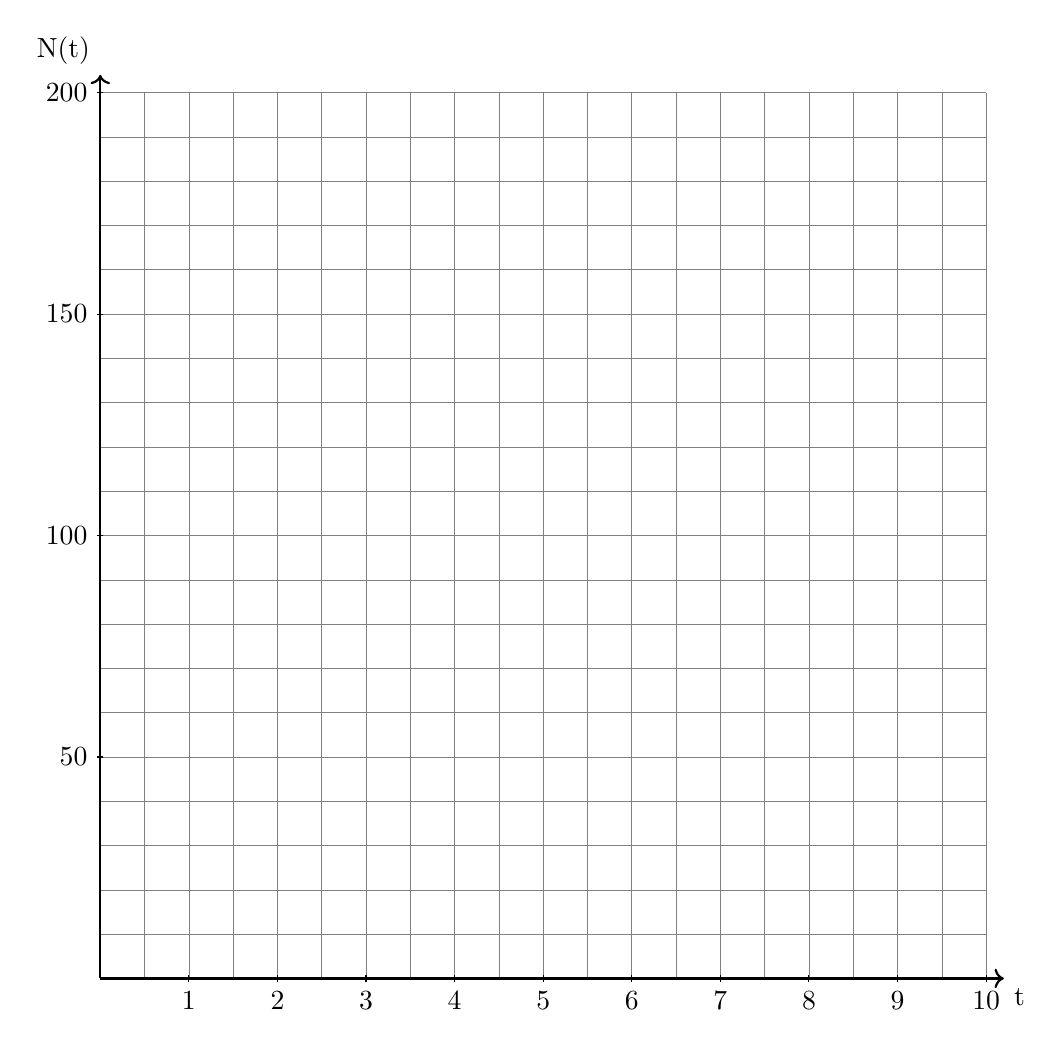
\begin{tikzpicture}[scale=4.5/4]
    \draw[step=0.5cm,gray,very thin] (0,0) grid (10,10);
    \draw[thick,->] (0,0) -- (10.2,0) node[anchor=north west] {t};
    \draw[thick,->] (0,0) -- (0,10.2) node[anchor=south east] {N(t)};
    \foreach \x in {1,2,3,4,5,6,7,8,9,10} \draw (\x cm,1pt) -- (\x cm,-1pt) node[anchor=north] {$\x$};
    \foreach \y in {2.5} \draw (1pt,\y cm) -- (-1pt,\y cm) node[anchor=east] {50};
    \foreach \y in {5} \draw (1pt,\y cm) -- (-1pt,\y cm) node[anchor=east] {100};
    \foreach \y in {7.5} \draw (1pt,\y cm) -- (-1pt,\y cm) node[anchor=east] {150};
    \foreach \y in {10} \draw (1pt,\y cm) -- (-1pt,\y cm) node[anchor=east] {200};
    \end{tikzpicture}
\end{center}
To the \emph{nearest hour}, $t$, when will the two drugs be at equal levels?\\*[0.5in]
When will $55$ milligrams of drug $B$ remain, to the \emph{nearest tenth of an hour}? 
\newpage

\item Sketch a graph with the following characteristics: 
\begin{itemize}
\item three real zeros
\item as $x \rightarrow + \infty$, $f(x) \rightarrow - \infty$
\item as $x \rightarrow - \infty$, $f(x) \rightarrow + \infty$
\end{itemize}
\begin{center}
    \begin{tikzpicture}[scale=2/4]
    \draw[thick,<->] (-7.5,0) -- (7.5,0) node[anchor=north west] {\textbf{x}};
    \draw[thick,<->] (0,-7.5) -- (0,7.5) node[anchor=south east] {\textbf{y}};
    \end{tikzpicture}
\end{center} %Alg2 Regents Jun2016 MC


\item Sketch a graph with the following characteristics: 
\begin{itemize}
\item polynomial function of order four
\item a positive leading coefficient
\item four real zeros
\end{itemize}
\begin{center}
    \begin{tikzpicture}[scale=2/4]
    \draw[thick,<->] (-7.5,0) -- (7.5,0) node[anchor=north west] {\textbf{x}};
    \draw[thick,<->] (0,-7.5) -- (0,7.5) node[anchor=south east] {\textbf{y}};
    \end{tikzpicture}
\end{center}

\newpage

\item For each polynomial graph, state 
\begin{enumerate}
\item its degree,
\item how many distinct zeros it has, and
\item the sign of its leading coefficient.
\end{enumerate}

    \begin{tikzpicture}[scale=2/4]
    %\draw[step=1cm,gray,very thin] (-7,-7) grid (7,7);
    \draw[thick,<->] (-7.5,0) -- (7.5,0) node[anchor=north west] {\textbf{x}};
    \draw[thick,<->] (0,-7.5) -- (0,7.5) node[anchor=south east] {\textbf{y}};
    %\foreach \x in {-6, -4, -2, 2, 4, 6} \draw (\x cm,1pt) -- (\x cm,-1pt) node[anchor=north] {$\x$};
    %\foreach \y in {5} \draw (1pt,\y cm) -- (-1pt,\y cm) node[anchor=east] {50}; %{$\y$};
    \tkzInit[xmin=-6,xmax=6,ymin=-7,ymax=7,ystep=1]   
    \tkzFct[color=black,thick,<->,domain = -4.3:5.2] {-0.1*(x+3)*(x)*(x-4)};
    \end{tikzpicture}
    \begin{tikzpicture}[scale=2/4]
    %\draw[step=1cm,gray,very thin] (-7,-7) grid (7,7);
    \draw[thick,<->] (-7.5,0) -- (7.5,0) node[anchor=north west] {\textbf{x}};
    \draw[thick,<->] (0,-7.5) -- (0,7.5) node[anchor=south east] {\textbf{y}};
    %\foreach \x in {-6, -4, -2, 2, 4, 6} \draw (\x cm,1pt) -- (\x cm,-1pt) node[anchor=north] {$\x$};
    %\foreach \y in {5} \draw (1pt,\y cm) -- (-1pt,\y cm) node[anchor=east] {50}; %{$\y$};
    \tkzInit[xmin=-6,xmax=6,ymin=-7,ymax=7,ystep=1]   
    \tkzFct[color=black,thick,<->,domain = -5.3:4.2] {-0.05*(x+5)*(x+3)*(x-1)*(x-4)};
    \end{tikzpicture}
\\[30pt]
    \begin{tikzpicture}[scale=2/4]
    %\draw[step=1cm,gray,very thin] (-7,-7) grid (7,7);
    \draw[thick,<->] (-7.5,0) -- (7.5,0) node[anchor=north west] {\textbf{x}};
    \draw[thick,<->] (0,-7.5) -- (0,7.5) node[anchor=south east] {\textbf{y}};
    %\foreach \x in {-6, -4, -2, 2, 4, 6} \draw (\x cm,1pt) -- (\x cm,-1pt) node[anchor=north] {$\x$};
    %\foreach \y in {5} \draw (1pt,\y cm) -- (-1pt,\y cm) node[anchor=east] {50}; %{$\y$};
    \tkzInit[xmin=-6,xmax=6,ymin=-7,ymax=7,ystep=1]   
    \tkzFct[color=black,thick,<->,domain = -1.3:5.2] {-0.5*(x-2)*(x-2)};
    \end{tikzpicture}
    \begin{tikzpicture}[scale=2/4]
    %\draw[step=1cm,gray,very thin] (-7,-7) grid (7,7);
    \draw[thick,<->] (-7.5,0) -- (7.5,0) node[anchor=north west] {\textbf{x}};
    \draw[thick,<->] (0,-7.5) -- (0,7.5) node[anchor=south east] {\textbf{y}};
    %\foreach \x in {-6, -4, -2, 2, 4, 6} \draw (\x cm,1pt) -- (\x cm,-1pt) node[anchor=north] {$\x$};
    %\foreach \y in {5} \draw (1pt,\y cm) -- (-1pt,\y cm) node[anchor=east] {50}; %{$\y$};
    \tkzInit[xmin=-6,xmax=6,ymin=-7,ymax=7,ystep=1]   
    \tkzFct[color=black,thick,<->,domain = -3.3:5.2] {0.05*(x*x*x*x-3*x*x*x-9*x*x+10*x+20)};
    \end{tikzpicture}


\newpage


\item If $g(c)=1-c^2$ and $m(c)=c+1$, then which statement is \emph{not} true?
\begin{enumerate}
    \item $g(c) \bullet m(c) = 1+c-c^2-c^3$
    \item $g(c) + m(c) = 2+c-c^2$
    \item $m(c) - g(c) = c+c^2$
    \item $\displaystyle \frac{m(c)}{g(c)} = \frac{-1}{1-c}$
\end{enumerate} %Regents Alg2 Jun2016


\item Solve for $x$: $\displaystyle \frac{1}{x} - \frac{1}{3} =-\frac{1}{3x}$\\[10pt]%Alg2 Regents Jun2016
Solve with a calculator by graphing the left-hand side as $\displaystyle y1=\frac{1}{x} - \frac{1}{3}$ and the right hand side as $y2=-\frac{1}{3x}$. Then use the calculator graph-solve function.\\[1in]
To get full credit, show work by sketching the graph. Mark the intersection clearly with the $x$ value. Write ``graphical solution."
\begin{center}
    \begin{tikzpicture}[scale=3/4]
    \draw[thick,<->] (-7.5,0) -- (7.5,0) node[anchor=north west] {\textbf{x}};
    \draw[thick,<->] (0,-7.5) -- (0,7.5); %node[anchor=south east] {\textbf{y}};
    \end{tikzpicture}
\end{center}

\newpage

\end{enumerate}
\end{document}

\item What is the expression $6xi^3(-4xi+5)$ is equivalent to?  %Alg2 Regents Jun2017 multiple choice

\item Simplify the expression $(3k - 2i)^2$, where $i$ is the imaginary unit. %Alg2 Regents Aug2017

